

\part{Flutkatastrophe 1953}
\section{Ablauf}
\newpage
\section{Folgen}
\newpage
\section{Wiederaufbau}
\newpage

\part{Delta Werke}
\section{Überblick}
\newpage
\section{Oosterschelde-Sturmflutwehr}
\newpage
\section{Maeslant-Sturmflutwehr}
\newpage
\section{Zukünftig geplante Erweiterungen}
\newpage

\part{Informierung der Bevölkerung}
\section{Notfallplan}
\subsection{Risikokarte}
Test 1 zu 1 von quelle:
TODO
QUELLE: $http://risicokaart.nl/de/informatie_over_risicos/overstroming$
\newline\newline
\textnormal{Die Risikokarte enthält Informationen über die Hochwassergefahr in den Niederlanden. 
Die Karte zeigt, wie hoch das Wasser in Ihrem Wohnort steigen kann und welche höher gelegenen Gebiete sicher sind.
}

\textnormal{\newline\bfseries Sie können sich auf das Hochwasser vorbereiten. 
Folgendes sollten Sie bereithalten:}
 
\begin{itemize}  
\item Ein Notpaket
\item Adressen, die Sie im Notfall aufsuchen können
\item Die Anfahrtsrouten zu diesen Adressen
\end{itemize}  

\textnormal{\newline\bfseries Wenn Hochwasser droht}
\newline
\textnormal{Sie werden mit Hilfe von lokalen Rundfunk- und Fernsehsendern, 
Alarmsirenen, SMS-Mitteilungen oder über Lautsprecherwagen der Polizei
 oder Feuerwehr gewarnt. Gehen Sie dann wie folgt vor:}
\begin{itemize}  
\item Schalten Sie den Radiosender für den Katastrophenfall ein und informieren Sie sich, falls möglich, 
auf der Website Ihrer Kommune oder unter www.crisis.nl über die aktuellen Entwicklungen.
\item Befolgen Sie die Anweisungen der Behörden und Einsatzdienste.
\end{itemize}  
\textnormal{\newline\bfseries Wenn Sie Ihre Wohnung verlassen müssen}
\begin{itemize}  
 \item   Sperren Sie Gas, Wasser und Strom ab.
\item    Nehmen Sie nur das Allerwichtigste mit (Bargeld, Medikamente und Kopien von Ausweisen und Versicherungspolicen).
\item    Schließen Sie die Wohnungstür ab.
 \item   Legen Sie Sandsäcke vor Türen und Fenster.
 \item   Vergewissern Sie sich, dass Ihre Nachbarn von der Evakuierung wissen.
\item    Tragen Sie festes Schuhwerk und wasserdichte Kleidung.
\item    Wenn Sie das Auto nehmen, legen Sie Sandsäcke vor Türen und Fenster Ihres Hauses und nehmen Sie Folgendes mit:
\item    Ihr Notpaket
\item    Ihre Haustiere und Futter/Wasser für die Tiere
\item    Einen Campingkocher mit zusätzlichem Brennstoff (Gas, Benzin), Töpfe und Essgeschirr
 \item   Eine Trillerpfeife (um Hilfe zu rufen)
 \item   Ein Tau und eine Plastikplane, mit der Sie einen Unterschlupf bauen können
 \item   Reservekraftstoff für Ihr Auto
\end{itemize}  
\textnormal{\newline\bfseries Wenn Sie die Wohnung nicht verlassen können}
\begin{itemize}  
   \item Begeben Sie sich mit Ihrem Notpaket an den höchsten Punkt in Ihrem Haus.
   \item Hängen Sie ein weißes Laken aus dem Fenster, um den Rettungskräften zu signalisieren, dass sich noch Personen im Haus befinden.
  \item  Helfen Sie anderen – wenn hierfür Zeit ist – bei den Notmaßnahmen und bieten Sie anderen sicheren Unterschlupf bei Ihnen an, wenn dies möglich ist.
\end{itemize}  
\textnormal{\newline\bfseries Während des Hochwassers}
\begin{itemize}  
  \item  Schalten Sie den Radiosender für Katastrophenfälle ein.
   \item Befolgen Sie alle Anweisungen.
  \item  Begeben Sie sich auf eine sichere Anhöhe und bleiben Sie dort. Warten Sie auf Hilfe.
 \item   Wenn für Ihre eigene Sicherheit gesorgt ist, helfen Sie Menschen in Ihrer Umgebung, die Hilfe benötigen.
  \item  Waten oder fahren Sie nicht durch das Wasser. Schnell fließendes Wasser, das mehr als knöcheltief ist, kann Sie leicht erfassen und mit sich reißen.
\end{itemize}   
\textnormal{Die folgende Übersicht zeigt, was Sie bei welchen 
Wasserständen noch tun können.}
\newline
\textnormal{\newline\bfseries Wasserstande Was können Sie selbst tun?}
\newline
\begin{tabular}[]{l p{10cm}}
0 - 20 cm &
Bringen Sie wichtige Gegenstände an einem hohen und trockenen Ort in Sicherheit. 
\newline Schützen Sie Ihren Besitz vor Schäden (Sandsäcke).
\newline Autos können noch im Schritttempo fahren. 
\newline\\ 
20 - 50 cm &
Bringen Sie sich selbst, Ihre Familie und wichtige Gegenstände in Sicherheit.
\newline Personen, die Hilfe benötigen, können noch zu Fuß erreicht werden. Helfen Sie anderen Menschen, soweit es geht.
\newline\\
50 - 80 cm &
Militärfahrzeuge können noch fahren. Rettungskräfte können noch zu Ihnen gelangen.
\newline Bringen Sie sich selbst und Ihre Familie in Sicherheit.
\newline Prüfen Sie, ob Sie an einem sicheren Ort noch anderen helfen können.
\newline\\
80 cm - 2 m &
Im ersten Stock Ihres Hauses sind Sie in Sicherheit.
\newline Bringen Sie sich selbst und Ihre Familie in Sicherheit und nehmen Sie Ihre Notvorräte sowie das Radio und Batterien mit.
\newline Schalten Sie den Radiosender für Katastrophenfälle (Lokalsender) ein und befolgen Sie die Anweisungen der Rettungskräfte.
\newline\\
2 - 5 m &
Im zweiten Stock Ihres Hauses sind Sie in Sicherheit.
\newline Bringen Sie sich selbst und Ihre Familie in Sicherheit und nehmen Sie Ihre Notvorräte sowie das Radio und Batterien mit.
\newline Schalten Sie den rampenzender [Radiosender für Katastrophenfälle] ein und befolgen Sie die Anweisungen der Rettungskräfte.
\newline\\
über 5 m &
Begeben Sie sich mit Ihren Notvorräten an den höchsten Punkt in Ihrem Haus.
\newline Halten Sie sich in der Nähe eines Ausgangs oder auf dem Dach auf, so dass Sie für die Rettungskräfte (Boot oder Hubschrauber) erreichbar sind. 
\newline Hängen Sie ein weißes Laken aus dem Fenster, um den Rettungskräften zu signalisieren, dass sich noch Personen im Haus befinden.
\\
\end{tabular}
\newline\newline 
\textnormal{\newline\bfseries Nach dem Hochwasser}
\newline 
Sie werden informiert, wenn die Gefahr in Ihrer Wohngegend vorüber ist. Begeben Sie sich nicht auf eigene Faust dorthin.
\newline\newline


\section{Kampagnen} 
\newpage
\section{Umfragen}
\subsection{Fragenansicht}
Haben Sie Angst vor Überflutung? \newline
Do you fear flooding?\newline
\newline
Wenn Sie hören, wenn ein Damm in der nähe bricht, was würden sie machen?\newline
What would you do, if a damm near you broke?\newline
\newline
Sind sie schon mal von einem Dammbruch betroffen gewesen?\newline
Have you ever been affected by a breaking damm?\newline
\newline
Machen sie sich sorgen um die Globale Erwärmung?\newline
Are you concernd about Global Warming, concerning possible floods as result?\newline
\newline
Sind sie schon mal bei Sicherheitsmaßnahmen aufgeklärt worden?\newline
Have you ever been spoken to about the safety measures? \newline
\newline
Gibt es Sachen die man am Damm grundsätzlich nicht macht?\newline
Is there anything you simply don't do, whene you're at a damm?\newline
\newline
Gibt es Aberglauben / Bauerregeln gegenüber Dämmen?\newline
Are there any superstitions or folk sayings about dams?\newline
\newline
Was ist ihre allgemeine Meinung gegenüber dem Damm?\newline
What's your general meaning of damms?\newline
\newline
Wer bestimmt über den Damm / Volksabstimmung?, Zufrieden, mehr Mitspracherecht?\newline
Who desides what happens with the damms?\newline
Are you okay with the current situation?\newline
\newline
Was spielt die Gefahr der Überflutung im allgemeinen Leben?\newline
Which role do damms play in your daily live?\newline


\subsection{Auswertung}
 
\newpage
\part{Maßnahmen der Überflutung und des Klimawandels}
\section{Sicherheitsmassnahmen}  
Test 1 zu 1 von quelle:
\newline\newline
ie Behörden aller Ebenen – von den Kommunen über die Provinzen bis 
hin zum Staat – setzen sich gemeinsam für den Hochwasserschutz ein.
 Das niederländische Amt für Wasserwirtschaft (Rijkswaterstaat) und
  die Wasserwirtschaftsverbände warten und kontrollieren gemeinsam 
  Deiche, Dämme und Dünen. Für die Flüsse wird zusätzlicher Raum 
  geschaffen. Die Kommunen informieren und warnen die Bevölkerung.
   Gemeinsam mit den Einsatzdiensten (Polizei, Feuerwehr und 
   medizinische Rettungsdienste) üben die Behörden regelmäßig
    den Ernstfall. Die Pegelstände werden ununterbrochen überwacht, 
    so dass im Prinzip genügend Zeit bleibt, Maßnahmen zu ergreifen
     und die Bevölkerung zu warnen.    

 
\section{Multy-Layer Safety}
\url{http://www.oranjewoud.nl/sites/default/oranjewoud_files/3_32556.pdf}
\subsection{Schwimmende Häuser} \footnote{Quelle Schwimmende Häuser: \cite{schwimmende_haeuser}}
schwimmende Häuser
--> Stadt Rotterdam	(in zehn jahren viele schwimmende häuser in der stadt)
da Rotterdam unterhalb des Meeresspiegels
\newline\newline
Styropor als Schwimmkörper
\newline\newline
Leben mit den Gezeiten
--> innerhalb 12h wird pavillon um durchschnittlich 2.5 meter gehoben und wieder gesenkt
\newline\newline
TODO
Quelle: http://www.spiegel.de/wissenschaft/technik/klimawandel-in-holland-wohnen-in-ebbe-und-flut-haeusern-a-800897.html 
\subsection{Wurten}
 \url{http://de.wikipedia.org/wiki/Sturmflut_1962}
\subsection{Polder-Abschottung} \footnote{Polder Quelle: \cite{polder}}
zb in dijkdoorbraak
\subsection{Evakuierung}
\url{http://www.spiegel.de/panorama/deich-undicht-niederlande-in-not-a-807633.html}
\url{http://www.uni-muenster.de/NiederlandeNet/aktuelles/archiv/2012/januar/0106hochwasser.shtml}   

\newpage
\part{Klimaerwärmung}
\section{Anstieg des Meeresspiegels}\footnote{Anstieg des Meeresspiegels Quelle: \cite{meeresspiegel} \cite{meeresspiegel2}} 
letzten 6000 Jahre, 0.5 bis 1mm pro Jahr
\newline
letzten 3000 Jahre,  0,1 bis 0,2mm pro Jahr
\newline
letzten Jahrzehnten, 1 bis 2mm pro Jahr
\newline
seit 1993, 3mm pro Jahr
\newline

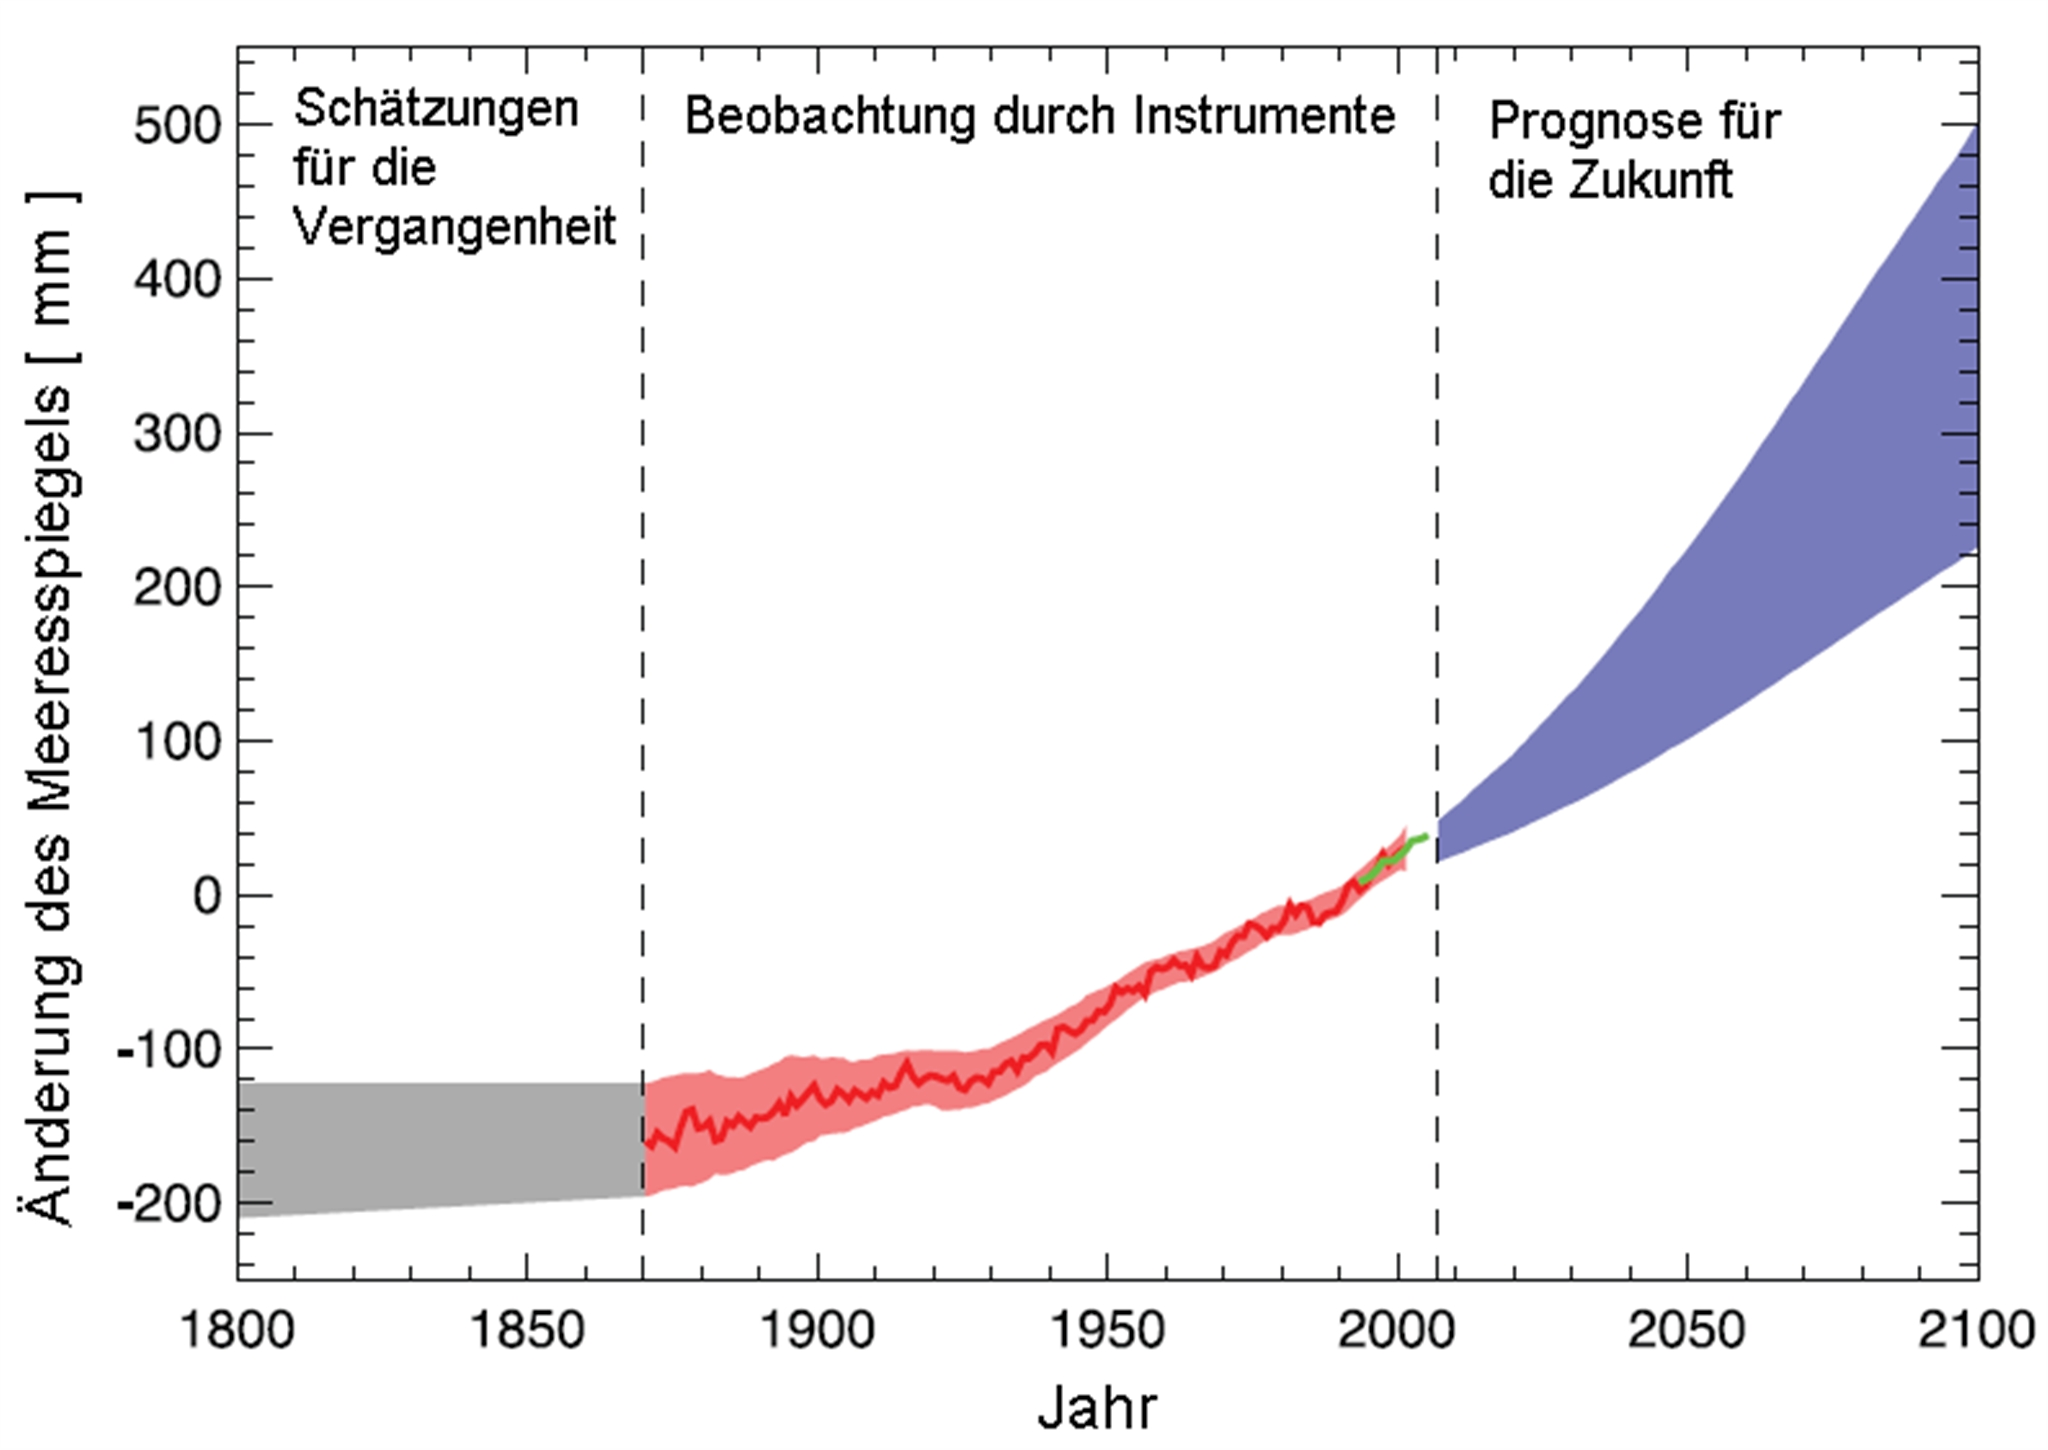
\includegraphics[width=1\textwidth]{images/anstieg.jpg}
\newline\newline


seit Anfang 20. Jahrhundert, 15
\newline
Da die Durchschnittstemperatur steigt, ,21. Jahrhundert = max 59 cm. 
+ Holland sinkt. (verkippen der Erdscholle) = um 10 cm bis zum 21. Jahrhundert
\newline
In Zukunft:  85 bis 130 cm pro Jahrhundert
\section{Holland kippt} \footnote{Holland kippt Quelle: \cite{meeresspiegel2}}
1 zu 1:\newline
Der Abstand zwischen Meeresspiegel und Meeresboden an der niederländischen Küste wird nicht 
nur durch den Meeresspiegelanstieg größer, sondern auch durch das Absinken des Meeresbodens. 
Rijkswaterstaat rechnet mit einer Absenkung des Bodens im niedrigen nordwestlichen Teil der Niederlande 
bis 2100 zwischen 0.5 und 2 Meter, der hohe südöstliche Teil wird einige Zentimeter steigen. 
Die Niederlande kippen somit langsam aber stetig in Richtung Nordsee. Diese natürliche Bodenbewegung 
ist im vergangenen Jahrhundert gleichmäßig verlaufen.
\newline
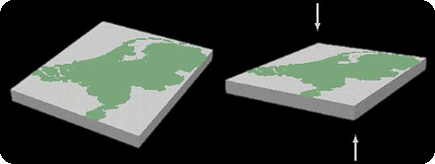
\includegraphics[width=1\textwidth]{images/niederlande_kippen.png}
\cite{kippen_bild} \text{Schema des Kippvorganges der Erdscholle}  

\section{Die Zukunft von Holland durch den Meeresspiegelanstieg} \footnote{Die Zukunft von Holland durch den Meeresspiegelanstieg Quelle: }
Wenn man davon ausgeht das der Meeresspiegel bis 2100 um 0.5 bis 2m steigt und Holland um 10 cm sinkt.
Ist zwischen 0.51m bis 2.1m alles möglich 
\newline
\newline
\color{red}  
TODO \newline
Landfläche Verlust bei 1m / 2m etc anstieg
Bewohner in Gefahr bei 1m/2n anstieg
--> Arbeit für Teil Zukunft
\newline
DelteWerke, wie viel halten sie aus?
Aufbau? Wie viel werden sie aushalten
\color{black}  
\newpage

\part{Worst-Case Szenario}
\section{Wirtschaftliche Folgen}
\newpage
\section{Personenschäden}
\newpage
\section{Wiederaufbau}
\newpage
\section{Bevölkerungsschutz}


 